\documentclass[border=6pt]{standalone}
\usepackage[T1]{fontenc}
\usepackage{lmodern,amsmath,amssymb,bm}
\usepackage{tikz}
\usetikzlibrary{arrows.meta,positioning,calc,shapes.geometric,decorations.pathmorphing,shadings}
\begin{document}
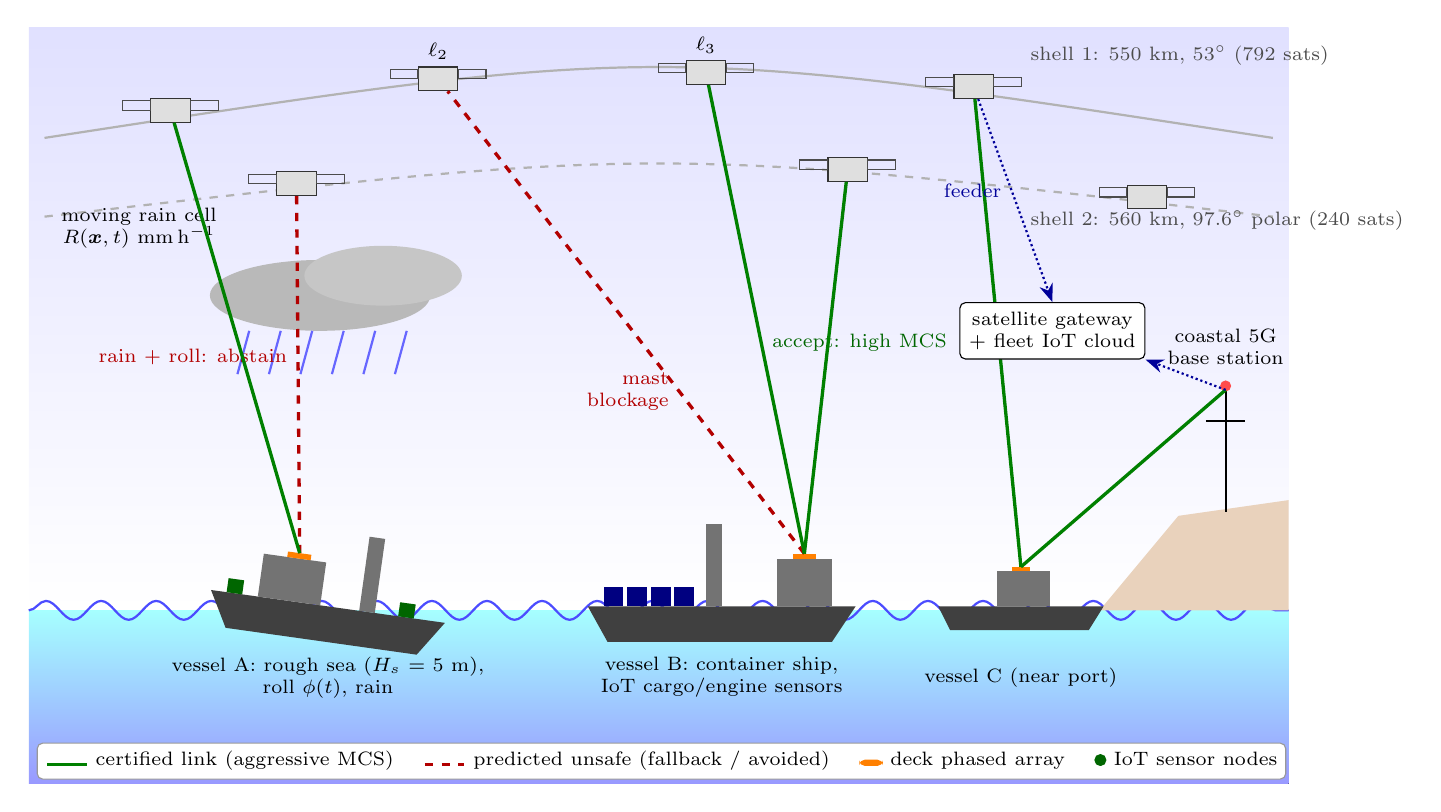
\begin{tikzpicture}[font=\sffamily\small, >=Stealth,
  sat/.style={draw=black!80, fill=gray!25, minimum width=5mm, minimum height=3mm, inner sep=0pt},
  ok/.style={very thick, green!50!black},
  no/.style={very thick, red!70!black, dashed},
  aux/.style={thick, blue!60!black, densely dotted}]
% ---------------- sky and shells
\fill[top color=blue!12, bottom color=white] (-8,1.2) rectangle (8,8.6);
\draw[gray!60, thick] (-7.8,7.2) .. controls (0,8.4) .. (7.8,7.2);
\draw[gray!60, thick, dashed] (-7.8,6.2) .. controls (0,7.1) .. (7.8,6.2);
\node[gray!60!black, font=\scriptsize, anchor=west] at (4.6,8.25) {shell 1: 550 km, 53$^\circ$ (792 sats)};
\node[gray!60!black, font=\scriptsize, anchor=west] at (4.6,6.15) {shell 2: 560 km, 97.6$^\circ$ polar (240 sats)};
\foreach \x/\y/\n in {-6.2/7.55/1,-2.8/7.95/2,0.6/8.03/3,4.0/7.85/4,-4.6/6.62/5,2.4/6.8/6,6.2/6.45/7}{
  \node[sat] (s\n) at (\x,\y) {};
  \draw[black!70] ($(s\n.west)+(-0.35,0)$) rectangle ($(s\n.west)+(0,0.12)$);
  \draw[black!70] ($(s\n.east)+(0,0)$) rectangle ($(s\n.east)+(0.35,0.12)$);
}
\node[font=\scriptsize] at (0.6,8.38) {$\ell_3$};
\node[font=\scriptsize] at (-2.8,8.3) {$\ell_2$};
% ---------------- sea
\fill[top color=cyan!35, bottom color=blue!40] (-8,-1.0) rectangle (8,1.2);
\draw[blue!70, thick, decorate, decoration={snake, amplitude=1.2mm, segment length=7mm}] (-8,1.2) -- (8,1.2);
% ---------------- coast with 5G base station and port
\fill[brown!35] (5.6,1.2) -- (8,1.2) -- (8,2.6) -- (6.6,2.4) -- cycle;
\draw[thick] (7.2,2.45) -- (7.2,4.0); \draw[thick] (6.95,3.6) -- (7.45,3.6);
\fill[red!70] (7.2,4.05) circle (0.07);
\node[font=\scriptsize, align=center] at (7.2,4.55) {coastal 5G\\ base station};
% ---------------- rain cell
\fill[gray!55] (-4.3,5.2) ellipse (1.4 and 0.45); \fill[gray!45] (-3.5,5.45) ellipse (1.0 and 0.38);
\foreach \x in {-5.2,-4.8,...,-3.0}{ \draw[blue!60, thick] (\x,4.75) -- ++(-0.15,-0.55); }
\node[font=\scriptsize, align=center] at (-6.6,6.05) {moving rain cell\\ $R(\bm x,t)$ mm\,h$^{-1}$};
% ---------------- vessel A (left, in storm, rolling)
\begin{scope}[shift={(-4.2,1.25)}, rotate=-8]
  \fill[black!75] (-1.5,0) -- (1.5,0) -- (1.2,-0.45) -- (-1.25,-0.45) -- cycle;
  \fill[black!55] (-0.9,0) rectangle (-0.1,0.55); \fill[black!55] (0.4,0) rectangle (0.6,0.95);
  \fill[orange] (-0.6,0.55) rectangle (-0.3,0.62);
  \coordinate (aA) at (-0.45,0.62); \coordinate (mA) at (0.5,0.95);
  \fill[green!40!black] (-1.3,0.0) rectangle (-1.1,0.18); \fill[green!40!black] (0.9,0.0) rectangle (1.1,0.18);
\end{scope}
\node[font=\scriptsize, align=center] at (-4.2,0.35) {vessel A: rough sea ($H_s$ = 5 m),\\ roll $\phi(t)$, rain};
% ---------------- vessel B (middle, calm)
\begin{scope}[shift={(0.8,1.25)}]
  \fill[black!75] (-1.7,0) -- (1.7,0) -- (1.4,-0.45) -- (-1.45,-0.45) -- cycle;
  \fill[black!55] (0.7,0) rectangle (1.4,0.6); \fill[black!55] (-0.2,0) rectangle (0.0,1.05);
  \foreach \xx in {-1.5,-1.2,-0.9,-0.6} {\fill[blue!50!black] (\xx,0) rectangle (\xx+0.25,0.25);}
  \fill[orange] (0.9,0.6) rectangle (1.2,0.67);
  \coordinate (aB) at (1.05,0.67); \coordinate (mB) at (-0.1,1.05);
\end{scope}
\node[font=\scriptsize, align=center] at (0.8,0.35) {vessel B: container ship,\\ IoT cargo/engine sensors};
% ---------------- vessel C (near port)
\begin{scope}[shift={(4.6,1.25)}, scale=0.75]
  \fill[black!75] (-1.4,0) -- (1.4,0) -- (1.15,-0.4) -- (-1.2,-0.4) -- cycle;
  \fill[black!55] (-0.4,0) rectangle (0.5,0.6);
  \fill[orange] (-0.15,0.6) rectangle (0.15,0.67);
  \coordinate (aC) at (0,0.67);
\end{scope}
\node[font=\scriptsize] at (4.6,0.35) {vessel C (near port)};
% ---------------- links
\draw[no] (aA) -- (s5) node[pos=0.55, left, font=\scriptsize, text=red!70!black] {rain + roll: abstain};
\draw[ok] (aA) -- (s1);
\draw[no] (aB) -- (s2) node[pos=0.35, left, font=\scriptsize, text=red!70!black, align=right] {mast\\ blockage};
\draw[ok] (aB) -- (s3) node[pos=0.45, right, font=\scriptsize, text=green!40!black] {accept: high MCS};
\draw[ok] (aB) -- (s6);
\draw[ok] (aC) -- (7.2,4.0);
\draw[ok] (aC) -- (s4);
% ---------------- ground segment
\node[draw, rounded corners=2pt, fill=white, font=\scriptsize, align=center] (gw) at (5.0,4.75) {satellite gateway\\ + fleet IoT cloud};
\draw[->, aux] (s4) -- node[pos=0.45, left, font=\scriptsize] {feeder} (gw.north);
\draw[->, aux] (7.2,4.0) -- (gw.south east);
% ---------------- legend
\node[draw=black!40, fill=white, rounded corners=2pt, anchor=south west, font=\scriptsize, align=left, inner sep=3pt] at (-7.9,-0.95) {%
\tikz{\draw[ok](0,0)--(0.5,0);} certified link (aggressive MCS) \quad
\tikz{\draw[no](0,0)--(0.5,0);} predicted unsafe (fallback / avoided) \quad
\tikz{\fill[orange](0,0) rectangle (0.3,0.08);} deck phased array \quad
\tikz{\fill[green!40!black](0,0) rectangle (0.15,0.15);} IoT sensor nodes};
\end{tikzpicture}
\end{document}
